\chapter{Obecná analýza a návrh}

Na základě požadavků na informační systém lze aplikaci rozdělit na dvě samostatné části. První je serverová aplikace s logickou složkou, jenž bude poskytovat \gls{api} pro klientské aplikace. Druhou nezbytnou část bude tvořit klientská webová aplikace využívající \gls{api} a obsahující vlastní logiku pro rendrování\footnote{Zde proces, při kterém z předem získaných dat vzniká grafické uživatelské rozhraní.} obsahu projektů.

Celkový předběžný návrh fungování aplikace \ref{pic:dia-deploy-sketch} zahrnuje tři uzly: databázový server, aplikační server a pracovní stanici uživatele. Databázový server je využíván pro udržování instancí databázových systémů, do kterých patří relační \gls{sql} databáze a dokumentová \gls{nosql} databáze. Aplikační server bude provozovat dvě navzájem komunikující aplikace -- webový server s veřejným \gls{api} a webový server poskytující uživatelské rozhraní. Server s veřejným \gls{api} může zabezpečeně komunikovat s databázovými systémy. Dané rozdělení zajistí případný vývoj klientských aplikací pro jiné platformy. Poslední uzel představuje pracovní stanici uživatele, na kterém bude v prohlížeči spuštěno uživatelské webové rozhraní, které bude komunikovat s vlastním webových serverem a \gls{api}.

\begin{fig:illustration}
   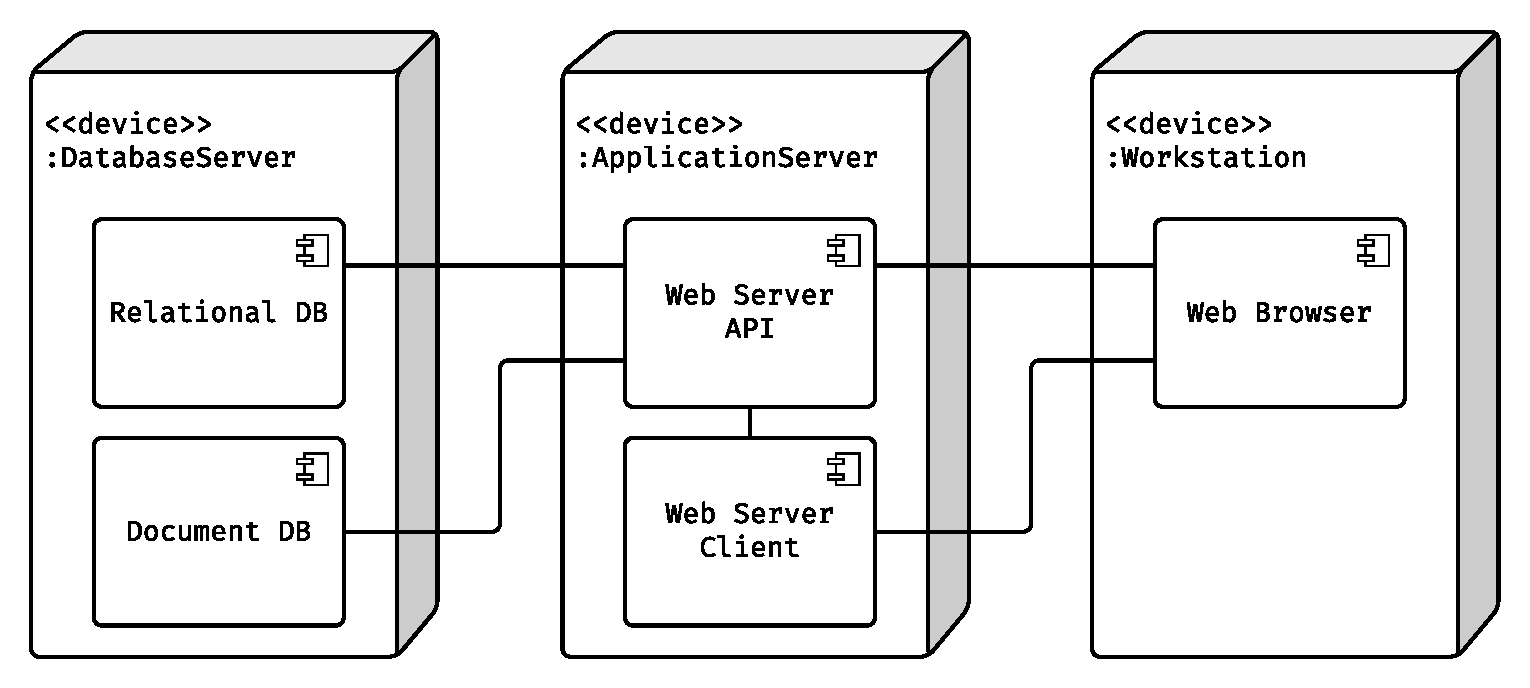
\includegraphics[width=1\textwidth]{images/dia-deploy-sketch.pdf}
   \caption{Návrh struktury uzlů a komponent, které jsou na nich spuštěny.}\label{pic:dia-deploy-sketch}
\end{fig:illustration}

Pro verzování obou aplikací bude využit \gls{vcs} Git -- jeden z nejpopulárnějších \gls{oss} \gls{vcs} v posledních letech~\cite{vcsG2}. Výhodou Git je jeho decentralizovanost, která je velice důležitá pro vývoj \gls{oss} aplikací, protože poskytuje nezávislost jednotlivým vývojářům.



% --------------------------------------------------------------------------------------------------
% Vybrané nástroje a technologie
% --------------------------------------------------------------------------------------------------


\section{Nástroje a technologie}

Kromě výše uvedeného nástroje pro správu verzí Git budou obě aplikace informačního systému využívat i další společné nástroje a technologie. Poslední část této kapitoly popisuje některé z nich s uvedením subjektivních důvodů, proč byly vybrány. Specifické nástroje, jenž byly zvoleny pro implementaci pouze serverové nebo klientské aplikace, budou podrobně popsány v kapitolách 4 a 5. 

\subsection{JavaScript}
Jako základní jazyk pro implementaci je vybrán JavaScript standardu ECMAScript 2016. Z hlediska klientské webové aplikace je to jediná efektivní možnost pro realizaci potřebné funkcionality. JavaScript na severu je spouštěn v NodeJS prostředí a byl zvolen pro přehlednost a jednotnost z hlediska využívaných knihoven.

\subsection{Yarn}
Správce balíčků je důležitou součástí každého většího projektu, poskytuje pohodlné rozhraní pro správu a využití knihoven třetích stran s případnou automatickou aktualizací závislostí. Pro jazyk JavaScript existuje několik správců, mezi které patří npm a Yarn. Dle osobních zkušeností byl vybrán Yarn, protože v posledních letech byl mnohem stabilnější z hlediska poskytované funkcionality.

\subsection{Prettier}
Prettier je nástroj zajištující kvalitu kódu z hlediska vizuální stránky. Kontroluje zdrojové kódy více než 12 jazyků a knihoven, mezi které patří například JavaScript, JSX, TypeScript, SCSS, HTML a JSON~\cite{prettier}, jež jsou využívány v implementaci \gls{is}.